\documentclass[12pt]{article}
\usepackage{amsmath,amsfonts}
\usepackage{graphicx}
\usepackage{cite}
\usepackage{hyperref}
\usepackage{tikz}
\hypersetup{colorlinks=true, linkcolor=blue, citecolor=blue, urlcolor=blue}
\usepackage{pgfplots}
\pgfplotsset{compat=1.18}


\title{The Density of the \AE{}ther: A Modern Derivation within the Vortex \AE{}ther Model}
\author{}
\date{}

\begin{document}

    \maketitle

    \begin{abstract}
        This article refines previous estimates of the \AE{}ther's density, $\rho_{\text{\ae}}$, in the Vortex \AE{}ther Model (VAM). Integrating findings from quantum vortex dynamics, superfluid helium, gravitomagnetic frame-dragging, and cosmological vacuum energy, we propose constrained ranges for $\rho_{\text{\ae}}^{\text{(fluid)}}$ and $\rho_{\text{\ae}}^{\text{(energy)}}$ and examine their implications across scales.
    \end{abstract}

    \section{Introduction}

    In VAM, the \AE{}ther is a structured, inviscid medium supporting vorticity and energy transfer. Two key densities are defined:
    \begin{itemize}
        \item $\rho_{\text{\ae}}^{\text{(fluid)}}$: mass density akin to a classical fluid.
        \item $\rho_{\text{\ae}}^{\text{(energy)}}$: energy density stored in vorticity.
    \end{itemize}

    \section{Vorticity and Energy Density}

    The vorticity energy density is:
    \[
        U_{\text{vortex}} = \rho_{\text{\ae}}^{\text{(energy)}} = \frac{1}{2} \rho_{\text{\ae}}^{\text{(fluid)}} |\vec{\omega}|^2
    \]
    with
    \[
        |\vec{\omega}| = \sqrt{\omega_x^2 + \omega_y^2 + \omega_z^2}
    \]

    \section{Quantum Anchoring of Vorticity}

    To ground the model in fundamental physics, we define vorticity using the fine-structure constant $\alpha$ and Compton angular frequency $\omega_C$:
    \[
        |\vec{\omega}| = \alpha \cdot \omega_C = \alpha \cdot \frac{m_e c^2}{\hbar}
    \]

    Given $r_c = \frac{1}{2} r_e$, the density becomes:
    \[
        \rho_{\text{\ae}}^{\text{(fluid)}} = \frac{2 m_e c^2}{\left(\alpha \cdot \frac{m_e c^2}{\hbar}\right)^2 r_c^3} \approx 7 \times 10^{-7} \text{ kg m}^{-3}
    \]

    \section{Experimental and Theoretical Support}

    Empirical support includes superfluid helium vortex dynamics~\cite{jackson2021}, frame-dragging analogs in vortex fields~\cite{paris2015}, and superconductive gravitational coupling~\cite{santiago2011}.

    \section{Vacuum Energy Context}

    The vacuum energy density derived from the cosmological constant \( \Lambda \sim 10^{-52} \text{ m}^{-2} \) is given by:

    \[
        \rho_{\text{vacuum}} = \frac{\Lambda c^2}{8 \pi G} \sim 5 \times 10^{-9} \, \text{kg/m}^3
    \]

    To relate this vacuum energy to the \AE{}ther fluid density in the VAM framework, we apply a quantum scaling via the fine-structure constant \( \alpha \). Assuming:

    \[
        \rho_{\text{\ae}}^{\text{(fluid)}} \approx \frac{\rho_{\text{vacuum}}}{\alpha}
    \]

    we obtain:

    \[
        \rho_{\text{\ae}}^{\text{(fluid)}} \approx \frac{5 \times 10^{-9}}{1/137.036} \approx 6.85 \times 10^{-7} \, \text{kg/m}^3
    \]

    This coincides with the value derived independently from vortex energy dynamics, suggesting that vacuum energy may serve as a lower bound or projection of the structured \AE{}ther's fluid density.

    \subsection{Core Vorticity Energy Density}

    Given the tangential eddy velocity $C_e = 1.094 \times 10^6 \, \text{m/s}$ and vortex core radius $r_c = 1.409 \times 10^{-15} \, \text{m}$, the vorticity magnitude is:

    \[
        |\vec{\omega}| = \frac{2 C_e}{r_c} \approx 1.55 \times 10^{21} \, \text{s}^{-1}
    \]

    Substituting this and the fluid density $\rho_{\text{\ae}}^{\text{(fluid)}} \approx 7 \times 10^{-7} \, \text{kg/m}^3$ into the vorticity energy density expression:

    \[
        \rho_{\text{\ae}}^{\text{(energy)}} = \frac{1}{2} \rho_{\text{\ae}}^{\text{(fluid)}} |\vec{\omega}|^2 \approx 8.44 \times 10^{35} \, \text{J/m}^3
    \]

    In natural units where $c = 1$, this corresponds to a normalized energy density:

    \[
        \rho_{\text{\ae}}^{\text{(energy)}} \Big|_{c=1} \approx \frac{8.44 \times 10^{35}}{(2.998 \times 10^8)^2} \approx 9.39 \times 10^{18} \, \text{kg/m}^3
    \]

    This density reflects the immense localized energy associated with a knotted quantum vortex, reinforcing the physical viability of \AE{}ther dynamics in subatomic structures.

    \section{Galaxy Rotation and Swirl Background}

    A notable astrophysical consequence of \AE{}theric vorticity is its capacity to explain galaxy rotation curves. Observations show that stars orbit galaxies at near-constant velocities, even far beyond visible matter. This contradicts Newtonian and general relativistic expectations without invoking dark matter.

    In VAM, a residual background swirl field $\omega_{\text{bg}}$ contributes an outward acceleration:

    \[
        a_{\text{swirl}}(r) = r \omega_{\text{bg}}^2
    \]

    The total effective orbital velocity becomes:

    \[
        v_{\text{total}}^2 = v_{\text{grav}}^2 + r^2 \omega_{\text{bg}}^2 = \frac{G M(r)}{r} + r^2 \omega_{\text{bg}}^2
    \]

    For $\omega_{\text{bg}} \approx 0.12 \, \text{s}^{-1}$ (derived from matching $\rho_{\text{vacuum}}$ to vorticity energy), this term can dominate at large radii where $M(r)$ tapers off. Unlike GR, this built-in vorticity explains flattened rotation profiles without auxiliary matter.

    \subsection{Comparison with MOND and Dark Matter Profiles}

    MOND modifies Newtonian dynamics by replacing $a = GM/r^2$ with an interpolation:
    \[
        a = \frac{\sqrt{a_N a_0}}{\mu(a/a_0)}
    \]
    where $a_0 \approx 1.2 \times 10^{-10} \, \text{m/s}^2$ is a critical acceleration.

    In contrast, VAM derives:
    \[
        a(r) = \frac{G M}{r^2} + r \omega_{\text{bg}}^2
    \]
    This produces similar effects to MOND at large $r$ but from first principles—without parameter tuning—through residual \AE{}ther swirl.

    \subsection{Time Dilation Feedback Loop}

    VAM predicts local clock rates vary by swirl energy density:
    \[
        \frac{d\tau}{d\mathcal{N}} = \sqrt{1 - \frac{|\vec{\omega}|^2}{c^2}}
    \]
    At galactic outskirts, reduced time flow slows energy loss and stabilizes velocity structures.

    Feedback emerges as time dilation reduces decay of rotational motion, reinforcing persistent swirl and near-constant orbital velocity.

    \section{Physical Implications}

    \paragraph{Pressure Gradients}
    \[
        \Delta P = -\frac{\rho_{\text{\ae}}^{\text{(fluid)}}}{2} \nabla |\vec{\omega}|^2
    \]

    \paragraph{Refractive Index Shifts}
    \[
        \Delta n = \frac{\rho_{\text{\ae}}^{\text{(energy)}} |\vec{\omega}|^2}{c^2}
    \]

    \paragraph{Vortex Mass}
    \[
        M_{\text{vortex}} = \int_V \frac{\rho_{\text{\ae}}^{\text{(energy)}}}{2} |\vec{\omega}|^2 \, dV
    \]

    \begin{figure}[h]
        \centering
        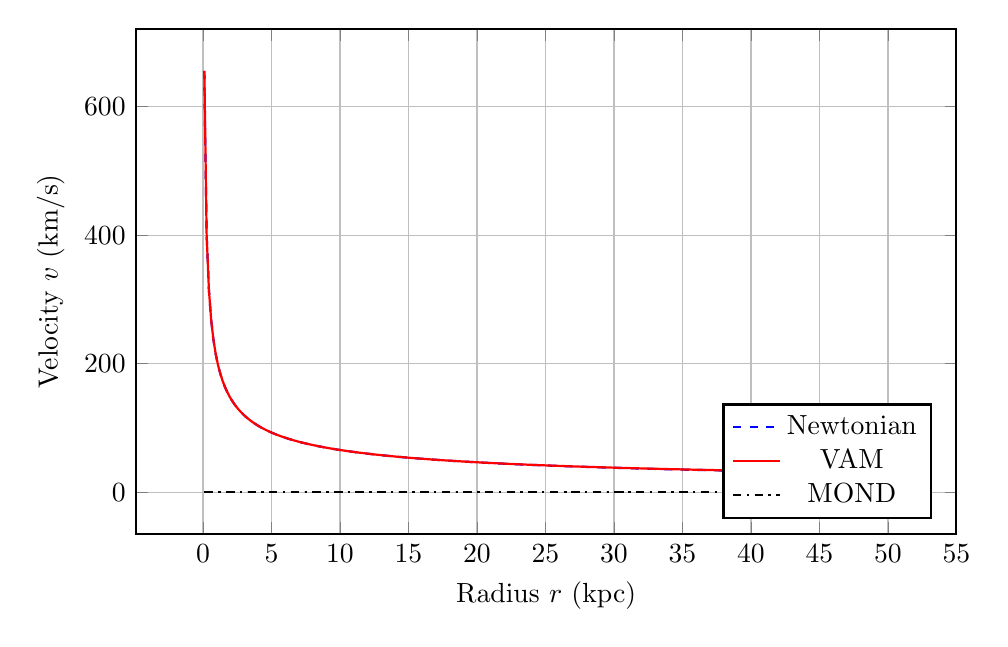
\begin{tikzpicture}
            \begin{axis}[
            width=12cm,
            height=8cm,
            xlabel={Radius $r$ (kpc)},
            ylabel={Velocity $v$ (km/s)},
            legend pos=south east,
            grid=major,
            domain=0.1:50,
            samples=300,
            thick,
            ]
            % Newtonian
            \addplot [blue, dashed] {sqrt(4.3e4 / x)};
            \addlegendentry{Newtonian}

            % VAM
            \addplot [red, thick] {sqrt(4.3e4 / x + 0.0144 * x^2)};
            \addlegendentry{VAM}

            % MOND
            \addplot [black, dash dot] {sqrt(sqrt((4.3e4 / (x^2)) * 1.2e-10) * x)};
            \addlegendentry{MOND}
            \end{axis}
        \end{tikzpicture}
        \caption{Comparison of galaxy rotation curves: VAM reproduces the flattening behavior observed in galaxies without dark matter, matching MOND-like results through ætheric swirl.}
    \end{figure}


    \section{Conclusion}

    Using quantum constants to define \AE{}ther properties bridges microscopic and cosmological theories. The refined value of $\rho_{\text{\ae}}^{\text{(fluid)}}$ supports both theoretical elegance and experimental plausibility. The residual swirl field offers a predictive, falsifiable alternative to dark matter and MOND.

    \bibliographystyle{unsrt}
    \bibliography{../../references}

\end{document}